\section{Introduction}~\label{sec:introduction}

Place recognition is a fundamental problem in autonomous navigation and mobile robotics, as it enables loop closure detection, global localization, and long-term map consistency. The goal is to generate compact yet highly discriminative scene descriptors that uniquely characterize a location while remaining invariant to viewpoint changes, illumination variations, seasonal effects, and dynamic objects. Designing such robust representations remains a central challenge in perception systems.
Early place recognition approaches relied on handcrafted visual descriptors such as SIFT~\cite{lowe1999object, Lowe04}, SURF~\cite{Bay2006, Bay2008346}, ORB~\cite{Rublee2011}, HOG \cite{Dalal2005}. The introduction of deep learning significantly improved robustness through convolutional architectures capable of learning hierarchical semantic representations. \\
A seminal contribution in this direction was NetVLAD~\cite{Relja2016}, which proposed a differentiable global descriptor aggregation layer enabling end-to-end training for large-scale place recognition. Although image-based global descriptors benefit from dense texture and strong contextual reasoning, they remain highly sensitive to illumination changes, shadows, weather conditions, and perceptual aliasing, where visually similar scenes correspond to distinct physical locations. \\
To overcome the limitations of purely appearance-based methods, LiDAR-based place recognition techniques operate directly on 3D point clouds, leveraging geometric structure instead of texture. Working in 3D space provides improved invariance to lighting conditions and enables more accurate discrimination of scene elements based on spatial configuration. The emergence of learning-based architectures such as PointNet~\cite{qi2017pointnetdeeplearningpoint} and PointNet++ \cite{qi2017pointnetdeephierarchicalfeature} enabled direct feature extraction from unordered point sets through permutation-invariant operations and hierarchical neighborhood aggregation.
Building upon these foundations, several works specifically targeted global 3D place recognition. PointNetVLAD~\cite{uy2018pointnetvladdeeppointcloud} combined PointNet-based feature extraction with a NetVLAD aggregation layer to learn discriminative global descriptors from raw point clouds. OverlapNet~\cite{ChenXieyuanli2020} proposed a LiDAR-based method that estimates overlap and relative yaw angle between scans, improving robustness in loop closure detection. More recently, MinkLoc3D \cite{komorowski2020minkloc3dpointcloudbased} leveraged sparse 3D convolutions within the Minkowski Engine framework to generate highly discriminative global descriptors directly from voxelized point clouds. These approaches demonstrated that learned 3D geometric descriptors significantly outperform handcrafted methods in large-scale outdoor localization. \\

In addition to global representations, learning-based local geometric descriptors such as FCGF (Fully Convolutional Geometric Features)~\cite{ChoyChristopher2019} and D3Feat~\cite{bai2020d3featjointlearningdense} have shown strong performance in point cloud matching and registration tasks. These models exploit sparse convolutional~\cite{tang2020searching} architectures and joint detector–descriptor learning~\cite{wang2021p2netjointdescriptiondetection} to enhance distinctiveness and repeatability in 3D space.
Despite these advances, relying exclusively on LiDAR data presents inherent challenges. Point clouds are sparse, irregular, and range-dependent, leading to uneven point distributions and reduced resolution at long distances. This dispersion weakens contextual modeling and limits semantic abstraction. While 3D geometry captures structural consistency, it often lacks appearance cues that help disambiguate perceptually similar environments.
Conversely, purely image-based descriptors provide rich texture and semantic information but suffer from sensitivity to illumination, weather, and dynamic elements. \\

\newpage

\begin{strip}
	\centering
	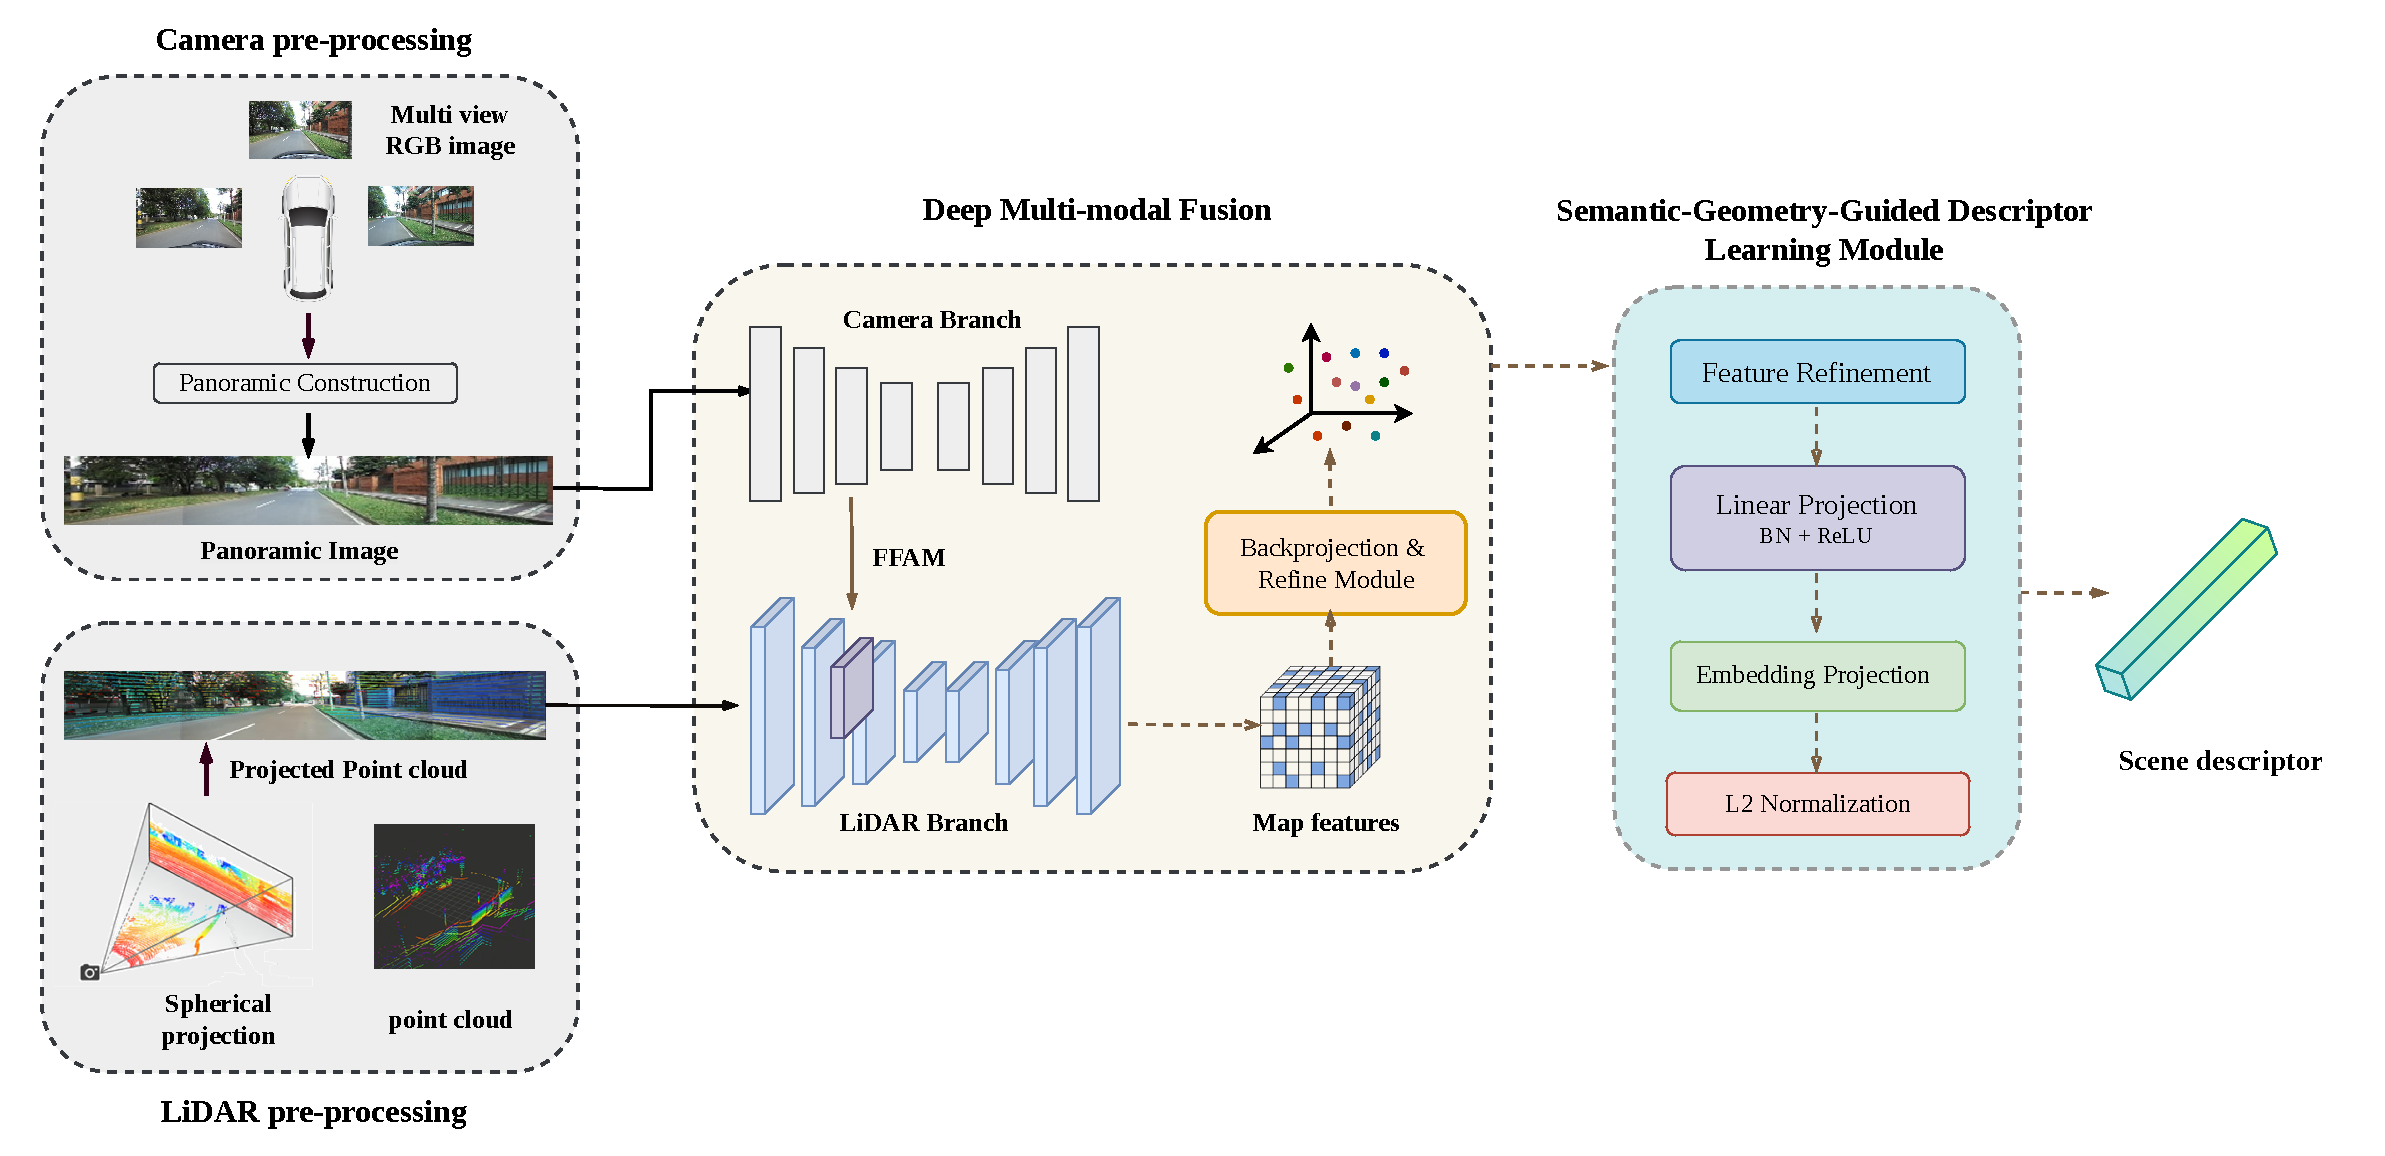
\includegraphics[width=\linewidth]{Figures/Pipeline-global-descriptor-multi-modal.pdf} 	
	\captionof{figure}{Main core of the proposed pipeline for generating global descriptors from multimodal data. The point cloud is projected onto the panoramic image, and both modalities are processed through a shared backbone to extract refined 3D features. A learnable global descriptor head aggregates these features into a compact embedding for place recognition.}	
	\label{fig:pipeline}
\end{strip}

Large-scale annotated datasets~\cite{behley2019semantickitti, nuscenes2019, SunKDCPTGZCCVHN20, eu_longterm_dataset} have highlighted the importance of semantic supervision for structured scene understanding; however, extracting semantically robust and globally discriminative representations from single modalities remains challenging.
These observations motivate multimodal fusion strategies that integrate LiDAR geometry with visual appearance. By leveraging the complementary nature of spatial structure and texture, multimodal approaches mitigate the modality-specific degradation factors that affect single-sensor systems. Nevertheless, multimodal fusion introduces additional challenges, including precise extrinsic calibration, accurate projection of 3D points onto the image plane, reliable cross-modal alignment, and increased computational complexity. \\

Motivated by the approach presented in~\cite{Snchez-Garca2025}, our pipeline as depicted in Fig~\ref{fig:pipeline} leverages panoramic images generated through a homography-based mosaicing of three stereo cameras, together with the corresponding LiDAR point cloud. The 3D measurements are projected onto the panoramic mosaic, effectively transforming geometric information into a 2D representation aligned with the image domain. In this manner, each pixel is enriched with geometric attributes associated with a spatial point prior to being processed by the semantic segmentation network. The output of the point cloud branch is subsequently re-projected into the 3D domain, following the strategy introduced in \cite{Lin2025},
In addition to semantic segmentation, we introduce a learnable global descriptor head that transforms refined 3D multimodal features into a compact and discriminative embedding suitable for place recognition. Unlike conventional approaches that rely on handcrafted pooling or intermediate logits, the proposed descriptor is extracted directly from the refined 3D feature space and aggregated through an attention-based global pooling mechanism. This design allows the network to selectively emphasize structurally stable and semantically informative regions while suppressing dynamic or less discriminative elements.

\begin{table*}[]
\caption{\scriptsize\MakeUppercase{Classical Handcrafted Local and Global Feature Descriptors for LiDAR Data}}
\label{tab:lidar-only-local-descriptors}
\begin{tabular}{|c|c|c|c|c|c|c|c|}
\hline
\rowcolor[HTML]{EFEFEF} 
\textbf{Ref.} & \textbf{Type} & \textbf{Descriptor} & \textbf{Main approach} & \textbf{\begin{tabular}[c]{@{}c@{}}Robust to\\ Viewpoint\end{tabular}} & \textbf{Semantic} & \textbf{Strengths} & \textbf{Limitation} \\ \hline
\multicolumn{1}{|c|}{\cite{Johnson1999}} &  & Handcrafted & \begin{tabular}[c]{@{}c@{}}Gradient-based keypoint \\ descriptor\end{tabular} & \begin{tabular}[c]{@{}c@{}}keypoint-\\ based\end{tabular} & X & \begin{tabular}[c]{@{}c@{}}Robust to illumination changes;\\  foundational for local matching\end{tabular} & \begin{tabular}[c]{@{}c@{}}Originally 2D; not designed \\ for raw 3D LiDAR; \\ computationally expensive\end{tabular} \\ \cline{1-1} \cline{3-8} 
\multicolumn{1}{|c|}{\cite{HungarConstanze2019}} &  & Handcrafted & \begin{tabular}[c]{@{}c@{}}Gradients of LiDAR intensity \\ for local description\end{tabular} & local frame & X & \begin{tabular}[c]{@{}c@{}}Exploits intensity information; \\ suitable for map-based localization\end{tabular} & \begin{tabular}[c]{@{}c@{}}Sensitive to intensity noise; \\ depends on sensor calibration\end{tabular} \\ \cline{1-1} \cline{3-8} 
\multicolumn{1}{|c|}{\cite{GuoJiadong2019}} &  & Handcrafted & \begin{tabular}[c]{@{}c@{}}Intensity distribution-based \\ descriptor\end{tabular} & Partial & X & \begin{tabular}[c]{@{}c@{}}Improves distinctiveness over \\ geometry-only descriptors\end{tabular} & \begin{tabular}[c]{@{}c@{}}Performance depends \\ on intensity consistency \\ across sessions\end{tabular} \\ \cline{1-1} \cline{3-8} 
\multicolumn{1}{|c|}{\cite{RusuRadu2009}} & \multirow{-4}{*}{Local} & \begin{tabular}[c]{@{}c@{}}Handcrafted \\ geometric\end{tabular} & \begin{tabular}[c]{@{}c@{}}Histogram of surface normals \\ and curvature relationships\end{tabular} & \begin{tabular}[c]{@{}c@{}}Local  \\ frame\end{tabular} & X & \begin{tabular}[c]{@{}c@{}}Fast; widely adopted; effective \\ for registration\end{tabular} & \begin{tabular}[c]{@{}c@{}}Sensitive to noise and \\ sparse point clouds; \\ limited discriminative power\end{tabular} \\ \hline
\multicolumn{1}{|c|}{\cite{Fan2021}} &  & Semantic & \begin{tabular}[c]{@{}c@{}}Histogram/topological structure \\ enriched with semantic classes\end{tabular} & $\checkmark$ & $\checkmark$ & \begin{tabular}[c]{@{}c@{}}Robust to structural \\ changes in urban scenes\end{tabular} & \begin{tabular}[c]{@{}c@{}}Depends on segmentation \\ accuracy\end{tabular} \\ \cline{1-1} \cline{3-8} 
\multicolumn{1}{|c|}{\cite{Liao2022}} &  & \begin{tabular}[c]{@{}c@{}}Topological-\\ semantic\end{tabular} & \begin{tabular}[c]{@{}c@{}}Graph-based topological \\ descriptor with semantic labels\end{tabular} & $\checkmark$ & $\checkmark$ & \begin{tabular}[c]{@{}c@{}}Robust to viewpoint variations; \\ interpretable structure\end{tabular} & \begin{tabular}[c]{@{}c@{}}Sensitive to semantic \\ misclassification\end{tabular} \\ \cline{1-1} \cline{3-8} 
\multicolumn{1}{|c|}{\cite{Cao2018}} &  & Geometric & \begin{tabular}[c]{@{}c@{}}Laser-based urban structural \\ descriptor\end{tabular} & $\checkmark$ & X & \begin{tabular}[c]{@{}c@{}}Effective in structured urban \\ environments\end{tabular} & \begin{tabular}[c]{@{}c@{}}Limited performance in \\ unstructured scenes\end{tabular} \\ \cline{1-1} \cline{3-8} 
\multicolumn{1}{|c|}{\cite{Wang2020}} &  & \begin{tabular}[c]{@{}c@{}}Projection-\\ based\end{tabular} & \begin{tabular}[c]{@{}c@{}}Polar image representation \\ (Iris-like encoding)\end{tabular} & $\checkmark$ & X & \begin{tabular}[c]{@{}c@{}}Rotation-invariant; compact \\ representation\end{tabular} & \begin{tabular}[c]{@{}c@{}}Sensitive to dynamic \\ changes\end{tabular} \\ \cline{1-1} \cline{3-8} 
\multicolumn{1}{|c|}{\cite{Fan2020}} &  & \begin{tabular}[c]{@{}c@{}}Segmentation-\\ based\end{tabular} & \begin{tabular}[c]{@{}c@{}}Egocentric segmentation-\\ driven structural descriptor\end{tabular} & $\checkmark$ & \begin{tabular}[c]{@{}c@{}}$\checkmark$ \\ partial\end{tabular} & \begin{tabular}[c]{@{}c@{}}Encodes structural context; \\ improved distinctiveness\end{tabular} & \begin{tabular}[c]{@{}c@{}}Dependent on reliable \\ segmentation\end{tabular} \\ \cline{1-1} \cline{3-8} 
\multicolumn{1}{|c|}{\cite{Li2021}} &  & Semantic & \begin{tabular}[c]{@{}c@{}}Extension of Scan Context \\ with semantic labels\end{tabular} & - & $\checkmark$ & \begin{tabular}[c]{@{}c@{}}High robustness to seasonal \\ and illumination changes; \\ efficient matching\end{tabular} & \begin{tabular}[c]{@{}c@{}}Increased complexity \\ compared  to Scan \\ Context\end{tabular} \\ \cline{1-1} \cline{3-8} 
\multicolumn{1}{|c|}{\cite{Xiang2021}} &  & \begin{tabular}[c]{@{}c@{}}Compact \\ geometric\end{tabular} & \begin{tabular}[c]{@{}c@{}}Compact 3D histogram-\\ based descriptor\end{tabular} & - & X & \begin{tabular}[c]{@{}c@{}}Very fast; suitable for indoor \\ mapping\end{tabular} & \begin{tabular}[c]{@{}c@{}}Lower discriminative power \\ in complex scenes\end{tabular} \\ \cline{1-1} \cline{3-8} 
\multicolumn{1}{|c|}{\cite{Zhou2022}} &  & Statistical & \begin{tabular}[c]{@{}c@{}}Normal distribution modeling \\ of geometric features\end{tabular} & $\checkmark$ & X & Compact and noise-robust & \begin{tabular}[c]{@{}c@{}}Sensitive to major \\ structural variations\end{tabular} \\ \cline{1-1} \cline{3-8} 
\multicolumn{1}{|c|}{\cite{Zhang2022}} &  & Geometric & \begin{tabular}[c]{@{}c@{}}Structural descriptor for \\ registration and LCD\end{tabular} & $\checkmark$ & X & \begin{tabular}[c]{@{}c@{}}Robust to occlusions; useful for \\ joint registration\end{tabular} & \begin{tabular}[c]{@{}c@{}}Moderate computational \\ cost\end{tabular} \\ \cline{1-1} \cline{3-8} 
\multicolumn{1}{|c|}{\cite{Wang2023}} &  & \begin{tabular}[c]{@{}c@{}}Projection-\\ based\end{tabular} & \begin{tabular}[c]{@{}c@{}}Double 3D-to-2D projection \\ strategy\end{tabular} & - & X & \begin{tabular}[c]{@{}c@{}}Higher discriminability than \\ single  projection methods\end{tabular} & \begin{tabular}[c]{@{}c@{}}Possible loss of fine 3D \\ information\end{tabular} \\ \cline{1-1} \cline{3-8} 
\multicolumn{1}{|c|}{\cite{Liu2023}} & \multirow{-11}{*}{Global} & Geometric & \begin{tabular}[c]{@{}c@{}}Enhanced Cartesian \\ histogram representation\end{tabular} & - & X & Lightweight; real-time capable & \begin{tabular}[c]{@{}c@{}}Sensitive to dynamic objects \\ and structural changes\end{tabular} \\ \hline
\end{tabular}
\end{table*}

To validate our framework, we conducted extensive experiments on the SemanticKITTI dataset, focusing on the object classes to be identified (vehicles, pedestrians, façades, and traffic signs). Our contributions are listed below: 

\begin{itemize}
    \item Building upon the VPA-Net architecture, we extend its multimodal fusion framework beyond dense semantic segmentation by introducing a learnable global descriptor head that extracts compact scene-level embeddings directly from refined 3D features.
    \item We integrate a homography-based panoramic mosaicing strategy to enlarge the field of view and strengthen multimodal spatial correspondence, enabling more context-aware feature learning.
    \item We unify dense semantic segmentation and global place-level representation within a single end-to-end trainable framework, bridging multimodal perception and scene retrieval without modifying the core backbone structure.
\end{itemize}

The remainder of this paper is structured as follows. Section II reviews the related work. Section III presents the details of our proposed network. Section IV discusses the experimental results. Conclusions and future work are drawn in the last section. 